\chapter{Introduction - clouds, climate and machine learning} \label{ch:introduction}

Clouds play a important role in the climate system. Both affecting the radiative budget and the hydrological cycle. \textit{Consist/Composed of liquid droplets, ice crystal or both.} Understanding how clouds form in the complex system of the atmosphere involves both knowledge about the large scale influence by the circulation and the small scale influenced by aerosols. To this day the micro-physics of all phases are not fully understood. Here mixed phase clouds, clouds consisting of both liquid and ice, \textit{proofs} to be the most difficult. Clouds and aerosols are acknowledged as the largest source to uncertainty in climate models and it \textit{remains unclear to which level of sophistication is required to model their effect on climate.} \textbf{Siter AR5}.
\\ \\
It is understood that cloud formation requires suitable aerosol and sufficient supersaturation. Aerosols include both gases and solid particles suspended in air.
They interact with the clouds by serving as particles which vapour ice can condensate or deposit upon. The different phases require different properties and are called \acrshort{ccn} for liquid droplets and \acrshort{inp} for ice crystals. Saturation is usually archived by a temperature decrease in rising air masses. Thus the stability of the atmosphere affect plays a key role for convective motions. 
%The negative temperature decreases by height is often referred to as the lapse rate, $\Gamma_{s, d}$. 
\\ \\ 
Growth processes are phase dependant. Liquid droplet grow by diffusion and later by collision and coalescence. At temperatures -38/-40 degrees \textbf{kilde} they will spontaneously freeze and could play the role as INP. If both phases are present in the a cloud saturation with respect to ice is higher than water. This causes droplets to evaporated and deposit on the ice crystals. This is called the Wegeron-Bergeron-Findeisen process. Clouds consisting sole of ice crystals first grow by deposition of vapour then by aggregation. 
\\ \\ 
Explain convection and fronts. Mention cumulus, status and cirrus clouds?
Feil og ikke nevne mer hydrologisk balance. Nevner i cloud schemes om endringer in tropical precip patterns. 
\\ \\ 

\\ \\ 
\section{Clouds in the current climate}
\begin{figure}
    \centering
    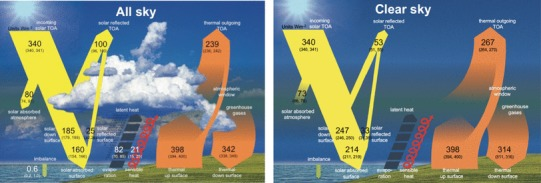
\includegraphics[scale = 7]{Chapter1_Intro/both_wild2019.jpg}
    \caption{The all-sky and the clear sky. Figure 14 Wild 2019. Ikke i bruk vennligst kommenter om denne er bedre enn den andre som viser differences mellom disse subplottene.}
    \label{fig:both_wild}
\end{figure}

\begin{figure}
    \centering
    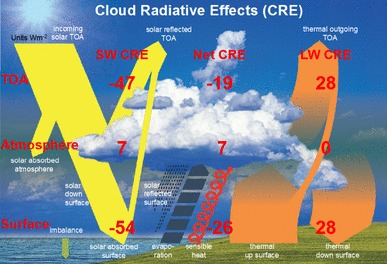
\includegraphics[scale = 7]{Chapter1_Intro/CRE_wild2019.jpg}
    \caption{Cloud radiative effect, CRE is the differece between the radiative components of the Clear sky radiative and the all sky. Cite this figure as fig 15 in Wild 2019}
    \label{fig:cre}
\end{figure}

Based on satellite and ground based measurements Wild et. al. 2019 have quantified the contribution of elements in the radiative budget. Subtracting the clear-sky from the all-sky climatology one can compute the cloud radiative effect, hereby referred to as CRE. This is shown in equations (\ref{eq:cre_sw}) and (\ref{eq:cre_lw}). Wild et. al. 2019 conclude with a reduction in shortwave radiation of $-47Wm^{-2}$ by clouds. In other words clouds reflect 50\% of the incoming solar radiation. Longwave component is $28Wm^{-2}$. This give a net CRE of $-19Wm^{-2}$. Proving that the net effects of clouds on the radiative budget is negative.The altitude along with the composition determines the radiative properties of the cloud.
\begin{equation} \label{eq:cre_sw}
    CRE_{sw} = SW\uparrow_{clear-sky} - SW\uparrow_{all-sky}
\end{equation}
\begin{equation} \label{eq:cre_lw}
    CRE_{lw} = LW\uparrow_{clear-sky} - LW\uparrow_{all-sky}
\end{equation}
\\
The physical properties of clouds causing the interaction with radiation is described below. Dense low level clouds reflect solar radiation. This is called the albedo effect of clouds. Albedo being the ratio between reflected to incoming radiation. The higher number concentrations of droplets in a cloud the higher the total surface area of droplets. The more radiation gets reflected. Clouds absorb longwave radiation and re-emits it. The absorbed radiation originates from the surface and is given by Stefan-Boltzmann forth-power law, see equation (\ref{eq:stefan-boltzmann}). High clouds have low temperatures and since the re-emitted flux is a function of the cloud temperature. The greenhouse effect increases with the height of the clouds.

\begin{equation} \label{eq:stefan-boltzmann}
    F = \sigma T ^4
\end{equation}

\section{Clouds in future climates}
\begin{figure}
    \centering
    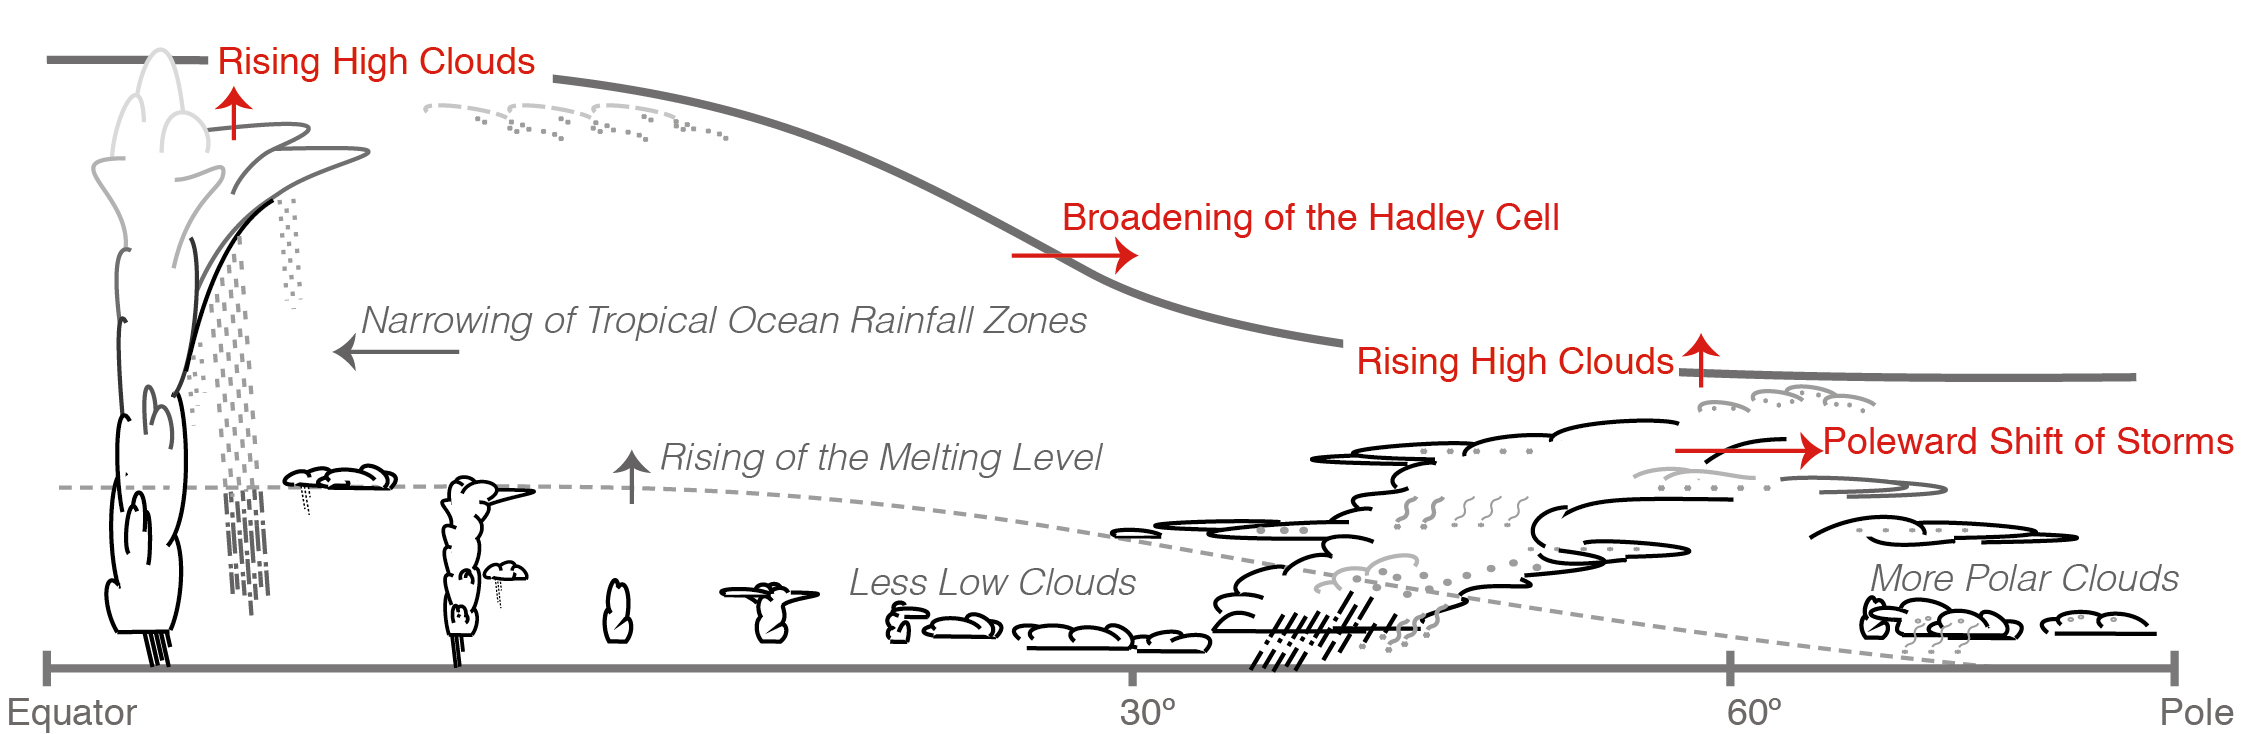
\includegraphics[scale = 0.8]{Chapter1_Intro/Fig7-11_ipcc.jpg}
    \caption{Cloud climatology in future climate. Developed based feedbacks in climate models, the different adjustments have different sikkerhet. Cite the fifth assessment report IPCC report.}
    \label{fig:cloud_scheme}
\end{figure}
\\ \\
Wild et. al. 2019 finds a imbalance of $0.6W m^{-2}$. This heat gets trapped in the earth system and cause the temperature increase. \textbf{define forcing}. The overall goal is to compute the climate sensitivity/equilibrium temperature as a function of forcing. 
\\ \\ 
The global temperature will keep rising until we have reached the equilibrium climate temperature. As the globe warms the climate changes. The IPCC suggest the following shift in cloud schemes. A broadening of the Hadley cell causes a poleward shift of storms. The albedo effect decrease at higher latitude. Moving the dense clouds further into the polar night, where only the greenhouse effect is present. The greenhouse effect of clouds still persist without sunlight leading to a net heating in the Arctic. Rising higher clouds causing a stronger greenhouse effect of clouds.
\\ \\
Aerosols can alter the cloud micro-physics and in term alter the radiative properties of the cloud. A polluted cloud gets extra \acrshort{ccn}, this results in more smaller droplets, as they share the available liquid. This increases the total surface area of the droplets and reflect more radiation. This will again led to a enhanced lifetime, since it takes longer for the droplets to reach precipitation size. If it does. On average 1 out of 10 cloud precipitate \textbf{kilde se skyfysikk bok}. As cloud precipitate they clean the air by removing particles.
\\ \\ 
Narrowing of the Tropical ocean rainfall zones causes a drier subtropics. Rising of the meltlayer may cause the ice crystals to melt resulting in more opaque clouds. Higher albedo. \textbf{read page 591-592 again.}
\\ \\
Cloud micro-physics is not yet fully understood. Along with the fact that clouds are formed a smaller scale then can be resolved in your average climate models. In order to get the contribution from subscale processes to mesoscale processes (weather) parametrizations are used. 
\\ \\
The parametization of subgridscale processes have gained more and more attention the last year. This has caused a larger spread in the uncertainty of climate models. \textbf{Add something more from model evaluation chapter in AR5.}
\\ \\ 
In this thesis I want to test if its possible to make a parametrization on total cloud cover based on macro-scale variables like humidity, surface temperature and pressure. Move away from the subgrid scale processes, by regressing historical observations against macro physical properties which affect clouds. The question remains: Is there be enough information in humidity, temperature and surface pressure to predict clouds in a time and space. 
\section{Deep Learning}
Due advances in hardware machine learning and available data have shown increasing potential. Machine learning have shown potential which transforms in a different fields ranging from self driving cars, face generation to cancer detection. \textbf{Kilder på de du nevner}. Also in geo-sciences this data driven approach continuous to gain more attention. Earth system monitoring provide a global view of variables for different meteorological systems. Neural network provide a flexible framework suitable across disciplines. They serve as universal approximates given a suitable hyper-param tuning and input data.
\\ \\ 
More and more data available becomes available from continuous earth system modelling. Based on estimates of future earth monitoring missions. Fig \ref{fig:data_volum_sat} shows the estimated available amount of data as a function of years.
\begin{figure}
    \centering
    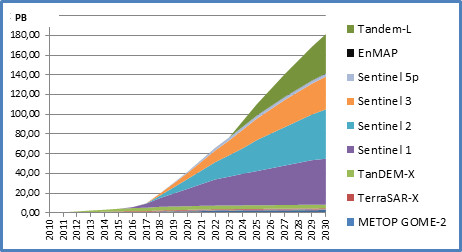
\includegraphics{Chapter1_Intro/Datenvolumen_D-SDA.jpg}
    \caption{Data volume. By the continuous earth system monitoring, meteorology/ climate science have progressed toward becoming a big data science. Observations are most used for verifying climate models and quantifying the current state of climate. }
    \label{fig:data_volum_sat}
\end{figure}
\href{https://www.dlr.de/eoc/en/desktopdefault.aspx/tabid-12632/22039_read-51751}{https://www.dlr.de/eoc/en/desktopdefault.aspx/tabid-12632/22039_read-51751}.
% https://www.dlr.de/eoc/en/desktopdefault.aspx/tabid-12632/22039_read-51751
\\ \\ 
\textit{Since applying artificial intelligence algorithms is quite new to geo-science I will give a brief historical remark on neural network and climate models.}
\\ \\ 
\textbf{Neural network}
\begin{figure}
    \centering
    \includegraphics[scale = 0.6]{Chapter1_Intro/untitled.png}
    \caption{Idea in ML.}
    \label{fig:ml}
\end{figure}
The main difference between the climate models and machine learning methods. \textbf{Stemmer ikke helt klimamodeller tunes også} ML models. are \textit{trained} and not explicitly programmed. The name neural network arise from neurons in the brain. As the field started in biologically
inspired computing. By learning we present the network with many examples/ samples of a given task. Hope the system can come up with the rules for automating such a task. In this thesis the rules are the physical relation of total cloud cover given temperature, pressure and humidity.
\\ \\
The depth in deep learning refers to the number of layers in the neural network.



\textbf{Kilde book chollet}
\\ \\
\textbf{Climate models}
\\ \\
There is a ongoing debate on what is intelligence. Traditionally a machine would be considered intelligent if it would beat a human at a given task. This has later been abandoned. The abilities a machine need to posses in order to beat a human in chess is completely different. A human needs X while the machine need Y. \textbf{kilde Chollet google} This will not be further discussed in this thesis since this is about task specific intelligence. Is it possible to train a network to gain sufficiently intelligent at the task of prediction European cloud cover?
\\ \\
Recurrent networks (LSTM) have been used for generating rainfall-runoff models (\textbf{kilde}) and for running air pollution forecasts and precipitation nowcasting models (\textbf{kilde}). Tapio Schneider at Caltech have ambitions to create a earth system model using machine learning. With his team of technologist from MIT and former employees of Microsoft and Google they hope to create a platform which can resolve clouds and hopefully reduce the climate sensitivity. 
\\ \\

\section{INSPO}
\begin{enumerate}
    \item No further adjustment is needed for a proper comparison.
\end{enumerate}

Siter Schubenau og si at satelitter definerer skyer basert på optical depth og at det derfor er nokså stor forskjellen på global gjennomsnittlig skydekket. I tillegg har man forskjeller på retrival algorithmns and sensors. 

\subsection{NOTES -- to be removed}
I dagen klima vet vi at skyer er vektig
Wild et al 2019 radiative budget.

Usikkerhet for fremtidig klima.
IPCC for klimafølsomhet og endringer i sky regimer. 

Manaby and Waetherall 1967 og (75?). første klimamodeller 
Hansen et al 1984.

Arrenius 1896 og tyndal 1861 fourier 1827.

cloud regimes from satelite images. What to expect in Europe. 

Figur forrig ipcc rapport. 

\begin{itemize}
    \item Sitere the earth machine. Si at machinlæring for stadig mer oppmerksomhet innenfor klimaforsning. 
    \item Snakke generelt om machine læring og artikkelen the measure of intelligence. 
    \item We’ll come back to this in
section 2.1.5.
\item To abbreviate the notation for the cross-entropy the loss function is used, so we can rewrite eq. (6) into
\item The distribution of values
by feature is shown in fig. 2.
\item Create correlation matrix using 
\item We will keep in mind both the scores of 0.743 and 0.782, serving
as fair baselines for a very simple, and slightly more sophisticated
regression fit, respectively.
\item Plotting R2 vs epoch, set ylim to 0,1. Not interresting to see where it learns.
\item Summaries the best five architecture 
\item A drawback of introducing more layers
is that it increases the complexity, and thereby the chance of
overfitting.

\end{itemize}